\hypertarget{sec:dsac-onto}{%
\chapter{Ontology-based Platform Development}\label{sec:dsac-onto}}
The platform presented in \cref{sec:dsac-composition-platform} offers a usable solution for the situational requirements of domain experts. As the second extension to this platform, following the Conversational-based Discovery and Composition Assistant, Domain Analyzer is presented in this chapter. Building on the DSAC platform, an ontology-based configuration mechanism is designed to implement a semantic layer to incorporates domain concepts and rules. The Domain Analyzer generates the Domain Reference Ontology serving as a comprehensive information object during the development, and the Domain Operation Ontology, which focuses on operational properties of the tool during the run time.

\hypertarget{sec:onto.analysis}{%
\section{Analysis}\label{sec:onto.analysis}}

Domain specificity and customization are key activities to support domain experts as co-designers of the situational applications. Although several studies underscore the importance of domain specificity, there are still few domain-specific platforms available for developing domain-specific mashups as situational solutions \autocite{Paterno2017b}. The scope of an \gls{eud} platform is defined as the range of supported tasks, spanning from general tasks common across many domains to tasks customized for a specific domain. Compared to generic tools, which have a technology-centric nature, domain-specific paradigms are more end-user-centric and have a better chance of improving productivity and increasing effectiveness \autocite{Daniel2014a}. Focusing on domain specificity when developing situational decision support solutions necessitates a comprehensive analysis and modeling of the domain. This approach also requires strategic planning on how to effectively incorporate domain knowledge into the final solution \autocite{Soi2014a}.  
In this section, we thoroughly analyze the domain specificity in \gls{eud} research domain. The following definitions provide relevant key terminologies: 

\begin{thesisdefinition}{Domain}{def:onto.domain}
A \gls{domain} is defined as a sphere of knowledge expressed with a set of concepts and activities that share common aspects that are known to the domain experts. These aspects pertain to the situation, performance, customer interaction, information processing, and more \autocite{Chemnitz2017}.
\end{thesisdefinition}


\begin{thesisdefinition}{Domain Model}{def:onto.domain-model}
The \gls{domain model} represents the requirements of the domain by identifying the domain concepts and processes as well as concrete data type, and information and control flow in the domain. This model results from collaboration between web developers and domain experts \autocite{Chemnitz2017}. Essentially, the \gls{domain model} captures the domain expert’s knowledge regarding the routine activities and concepts. For instance, in planning academic events, relevant concepts may include university, research groups, keynote speaker, and publication, while activities might involve identifying research groups, searching academic databases, and reserving venues. These activities lead us to identify the classes of components. The \gls{domain model} in this work is defined as an ontology, therefore the word \gls{domain model} and domain ontology will be used interchangeably.
\end{thesisdefinition}

\begin{thesisdefinition}{Ontology}{def:onto.ontology}
According to \autocite{Chemnitz2017} an \gls{ontology} is defined as a logical framework of terms to represent a specific domain of knowledge, encompassing the definitions of the relevant terms and their interrelationships.
\end{thesisdefinition}

\begin{thesisdefinition}{Domain-specific Mashup }{def:onto.domain-specific-mashup }
A \gls{Domain-specific Mashup Tool} is designed to meet the domain expert’s requirement  through domain-specific processes manipulating domain concepts \autocite{Casati2012}. This class of applications took the domain concepts and knowledge into account at different levels, such as interface design, component selection, functionality and mechanism definition \autocite{Gulliksen1995}. The \gls{domain model} should be applied at two levels of composition and \gls{ui} to fully address the domain specificity in composition tools. 
\end{thesisdefinition}

\vspace{-10pt}
\hypertarget{sec:onto.related-work}{%
\section{Related Work}\label{sec:onto.related-work}}
\vspace{10pt}
In this section we review and compare the existing approaches for ontology-based development and \gls{ontology} learning as a solution to address the domain specificity.

\vspace{-10pt}
\hypertarget{sec:related-work.onto}{%
\subsection{Ontology-based Development}\label{sec:related-work.onto}}
\vspace{10pt}

Unlike conventional software engineering methods, \gls{mde} fosters the modeling standards introduced by the OMG to
alleviate the methodology challenges of earlier approaches. In the early
1990s, domain-specific modeling emerged as a key part of Model-Driven
Engineering. This approach aims to facilitate software abstraction and
distinguish between domain and application requirements.
Domain-specific software development proposes enhanced efficiency and
maintenance, increased quality, and reduced development time and effort
\autocite{Jacobson2017}.

According to the survey conducted by \autocite{Zafar2024}, 
domain-specificity addressed in research studies can be categorized into
two classes of approaches: Metamodeling and \gls{dsl}.

A metamodeling tool provides a domain-specific modeling environment.
This technique leve es model transformations to translate the
source model into a refined domain-specific model. Despite successful
industrial usage, metamodeling faces some challenges. Most metamodeling
practices fail to capture the semantics of the domain and delegate this
task to the model compiler. \gls{dsl}s, on the other hand, are tailored to a
specific application domain, providing an abstraction representing the
domain concepts and terms. However, they often pose high complexity,
making them unusable for domain experts \autocite{Sosa2011}.

During the last decade, ontologies as a semantic web technology have
shown promising advances in domain-specific software and web
development. Ontologies can be used in various stages of application
development, ranging from requirement analysis to implementation.
Integrating such formal machine-readable models can significantly
promote interoperability, consistency, and reusability \autocite{Chhaya2020}. 
In the next section, ontology learning methods are reviewed.

\vspace{-10pt}
\hypertarget{sec:related-work.onto-learning}{%
\subsection{Ontology Learning}\label{sec:related-work.onto-learning}}
\vspace{10pt}

Ontology Learning refers to the process of constructing ontologies by extracting conceptual knowledge from unstructured text. This definition can be extended to include methods for enriching and adopting existing ontologies. Techniques for ontology learning are rooted in various fields such as natural language processing, machine learning, and data mining. These techniques differ based on the nature of the data used, whether unstructured or structured, as well as the intended application of the final ontology \autocite{Watrobski2020}. 
Generally, the ontology learning practices fall into one of the following categories: 

\begin{itemize}
\item
\emph{Shallow-parsing} approaches, categorized as linguistic,
statistical, and logic-based approaches. Linguistic approaches use
dependency analysis and syntactic rules to extract terms/concepts and
establish relationships between them. on the other hand, statistical
methods primarily rely on statistical metrics of the underlying corpus,
often disregarding semantics. These techniques heavily depend on term
frequency and probability \autocite{Mellal2021}. The logic-based
approaches leverage logical reasoning and formal logic such as inductive
logic programming \autocite{Asim2018}. Although shallow parsing methods are proven to be simple, easy to interpret and not data-intensive, they suffer from limitations related to scalability and handling large, domain-specific databases.


\item
\emph{Deep-learning} approaches.
The application of neural networks with multiple layers (deep
architectures) for the creation, refinement, or expansion of ontologies
has gained popularity during the recent years. Supervised methods like
\gls{cnn}, \gls{rnn}, and attention-based networks are used to extract terms,
concepts, and relationships. Word embedding approaches, such as
distributional embeddings using Word2Vec algorithms, are employed to
extend domain-specific concepts by identifying semantically related
terms. Deep learning-based approaches have shown promising results in
the field of\gls{ol}; however, in complex scenarios,
fine-tuning deep learning models requires significant computational
resources and machine learning expertise \autocite{Du2024}.


\item
\emph{\gls{llm}-based} approaches
In recent years, \gls{llm}s have made a significant
impact on the field of NLP in both academia and industry. \gls{llm}s are
mainly built on deep learning models and neural network architectures
\autocite{Crum2024}. These models are considered a specific type of
\gls{fm}s that are characterized by their pre-training on
massive datasets. \gls{fm}s can be fine-tuned to perform downstream tasks such
as text generation, translation, or text classification \autocite{Perera2024}.

The emergence of transformers in 2017, introduced by Google researchers
\autocite{Vaswani2017}, marked a significant turning point in the
field of natural language processing. Transformers employ a mechanism
known as \emph{Attention}, which was inspired by \gls{rnn}. This architecture allows for the development of
\textbf{encoder-only models}, like BERT\footnote{\url{https://huggingface.co/docs/transformers/en/model_doc/bert}}
(Bidirectional Encoder Representations from Transformers),
\textbf{encoder-decoder models}, and \textbf{decoder-only models}, such
as \gls{gpt}\footnote{\url{https://huggingface.co/docs/transformers/en/model_doc/openai-gpt}}
(Generative Pre-trained Transformer). The most dominant category of \gls{llm}s
is generated by decoder-only transformers, including models like \gls{gpt} or
PaLM, which are primarily used to generate new text \autocite{Perera2024}.


A limited number of researchers have addressed the role of \gls{llm}s in
ontology learning. LLM4OL \autocite{Giglou2023} introduced a
conceptual framework for performing OL tasks using \gls{llm}s. The authors
evaluated their work on 11 \gls{llm}s. In another study, an approach for
domain knowledge distillation using \gls{gpt}-based \gls{llm}s was proposed. This
method uses a seed ontology in the autonomous driving domain. However,
according to the authors, due to response randomness and the
``butterfly effect,'' the efficiency of a fully automated solution
cannot be guaranteed, and manual supervision remains necessary
\autocite{Tang2023}. The DRAGON-AI framework \autocite{Toro2023} uses
\gls{llm}s and \gls{rag} to generate ontology
components. The \gls{rag} technique produces the prompt as additional context
and feeds it to the \gls{llm}. The approach was tested with four \gls{llm}s and
provided valuable insights into the application of \gls{llm}s in OL.
According to the authors, the results indicated a moderate recall rate
for extraction and term/concept definition; therefore, \gls{llm}s should be
used cautiously.


During the rest of this chapter, the Domain Analyzer is reviewed in
detail. This tool is responsible for generating related ontologies and
applying domain knowledge.

\end{itemize}

\vspace{-10pt}
\hypertarget{sec:onto.domain-analyser}{%
\section{Domain Analyzer}\label{sec:onto.domain-analyser}}
\vspace{10pt}
Domain Analyzer develops the semantic layer as an abstraction layer to model and translate domain concepts and constraints into the components and business rules. The BPMN diagram in \cref{fig:onto-da}, models the domain analyzing process. The tasks are color-coding to distinguish between run time and development time tasks. The Domain Analyzer organizes tasks into two primary categories: Ontology Generation and Domain Configuration tasks.

\begin{figure}[hbt]
\hypertarget{fig:onto-da}{%
\centering
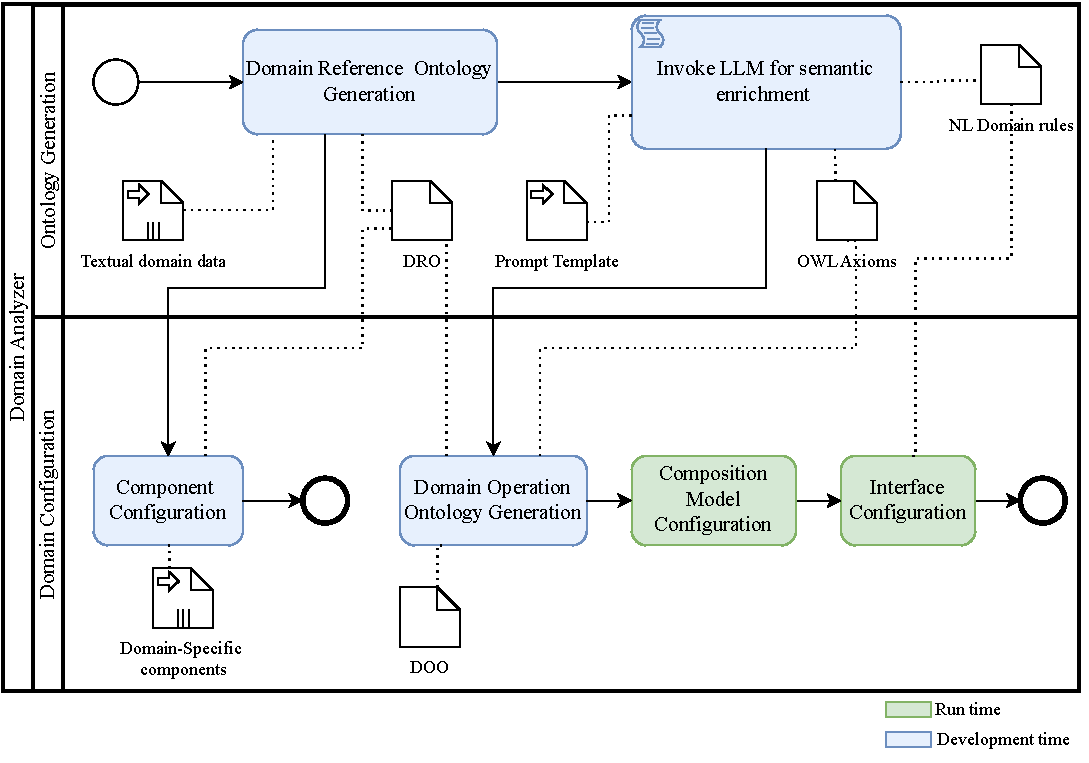
\includegraphics[width=0.85\textwidth]{../figures/MyFigures/DomainAnalyser.drawio.pdf}
\captionsetup{justification=centering}
\caption{Domain Analyzer Process Model}\label{fig:onto-da}
}
\end{figure}

The core element of this architecture is the ontology concept, which can
be formally defined as \(O\  = < \ C,H,\ R,\ A\  >\), where \(C\) is
defined as a set of concepts with \(H\) and \(R\) are the taxonomic
(hierarchical) and non-taxonomic (non-hierarchical) relations among
concepts, respectively. \(A\ \)represent set of axioms or rules.

Domain Analyzer differentiates between 2 types of ontologies, based on
their structure and the phase they are using in. The \gls{dro}) presents the domain's structural model and is used during
the development time. The Domain \gls{doo}, on the
other hand, is meant for semantic reasoning and computational purposes.
Using two distinct ontologies offers separation of concern and easy
domain adaptation \autocite{Haav2018}.

The process begins with the \emph{Domain Reference Ontology Generation}
task, which takes unstructured textual information as an input and
generates the \gls{dro}). This ontology serves as the foundational knowledge
base for the tool and provides the basis for its class diagram as a
structural model. Reference ontologies are primarily utilized during the
development time.

During the \emph{Component Configuration}, the \gls{dro}) is used for semantic
component annotations. These annotations are used during the component
discovery and composition.

The \emph{Semantic Enrichment} adds an additional semantics to the \gls{dro}
by incorporating the domain's operational constraints as ontological
axioms. These constrains, which are applied to domain concepts and
relationships, can subsequently be transformed into domain-specific
business rules. This task results in generating the \gls{doo}, which plays a
crucial role during the run time by defining dynamic domain,
particularly at the composition level. \gls{llm}s are integrated at this stage
for the generation of OWL axioms and business rules in natural language.
A structured prompt template is employed to guide the
\gls{llm}'s responses, enhancing consistency and reducing the
likelihood of model hallucinations \autocite{Perera2024}.
During the \emph{Domain Operation Ontology Generation}, the OWL axioms
in RDF/XML syntax is integrated into the \gls{dro}. The \emph{Composition
Model Configuration} process integrates the business rules, extracted
from \gls{doo} to the composition model as restrictions.

Typically, business rules are enforced at the backend and within the
composition level to ensure that the final outcome aligns with
domain-specific logic.

This whole process revolves around the concept of ontology learning,
which is employed to generate domain ontologies and integrate them into
the EUD tool. This integration aims to facilitate domain-specific
customizations and enable the reuse of knowledge within a particular
domain. Domain ontologies have the capacity to model a broad range of
concepts and knowledge within a given domain, some of which may not be
directly relevant to a specific use case. Therefore, the ontology
learning approach should be adapted to align with the specific
requirements of the application in which the knowledge will be utilized.
Throughout the next sections, the ontology learning, and domain
configuration process are reviewed in detail.

\vspace{-10pt}
\hypertarget{sec:ontology-gen}{%
\subsection{Ontology Generation}\label{sec:ontology-gen}}
\vspace{10pt} 	
The \gls{ol} process is summarized through a framework commonly referred to as the "ontology learning layer cake" (\cref{fig:onto-ol-cake}) \autocite{Asim2018}.

\begin{figure}[hbt]
\hypertarget{fig:onto-ol-cake}{%
\centering
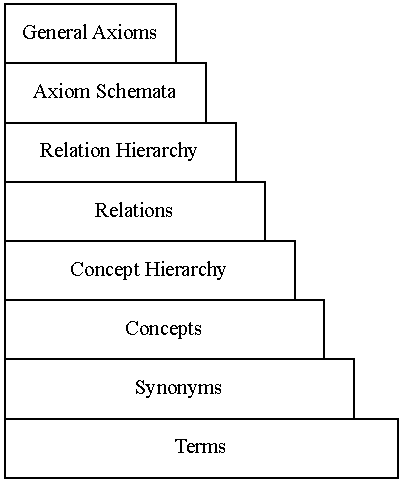
\includegraphics[width=0.85\textwidth]{../figures/MyFigures/OLLayerCake.drawio.pdf}
\captionsetup{justification=centering}
\caption{Ontology Learning Layer Cake \autocite{Wroblewska2012}}\label{fig:onto-ol-cake}
}
\end{figure}
The \cref{fig:onto-ol-cake} structures the required tasks for ontology acquisition into a hierarchical framework. In this structure, each upper layer is constructed upon the outputs of the preceding lower layers. The process begins with the creating the ontology taxonomy backbone by identifying terms and synonyms, which are then mapped to corresponding concepts. Establishing a hierarchical structure among these concepts is crucial for achieving the appropriate level of generalization for the relationships within the ontology. The four highest layers focus on extracting relations and forming a relational hierarchy as well as formulating arbitrary rules and axioms. 
In this work, we introduce a hybrid approach that incorporates lexical-syntactic patterns and statistical models such as Word2Vec for terms and relation extraction. Moreover, the  \gls{llm}s are leveraged as well to increase the performance in terms extraction and business rules generation. 
Lexical-syntactic patterns are structured rules that combine lexical items (words) with syntactic structures (grammar rules), primarily used for knowledge extraction and NLP purposes. These patterns indicate semantic relationships between terms and offer relatively good precision in relation extraction \autocite{Watrobski2020}. Hybrid methods benefit from the high precision of linguistic patterns and the flexibility of statistical models \autocite{Mellal2021}. 

Based on the OL Layer Cake structure, the following BPMN diagram presents the \gls{dro} and \gls{doo} generation process. 

\begin{figure}[hbt]
\hypertarget{fig:onto-onto-gen}{%
\centering
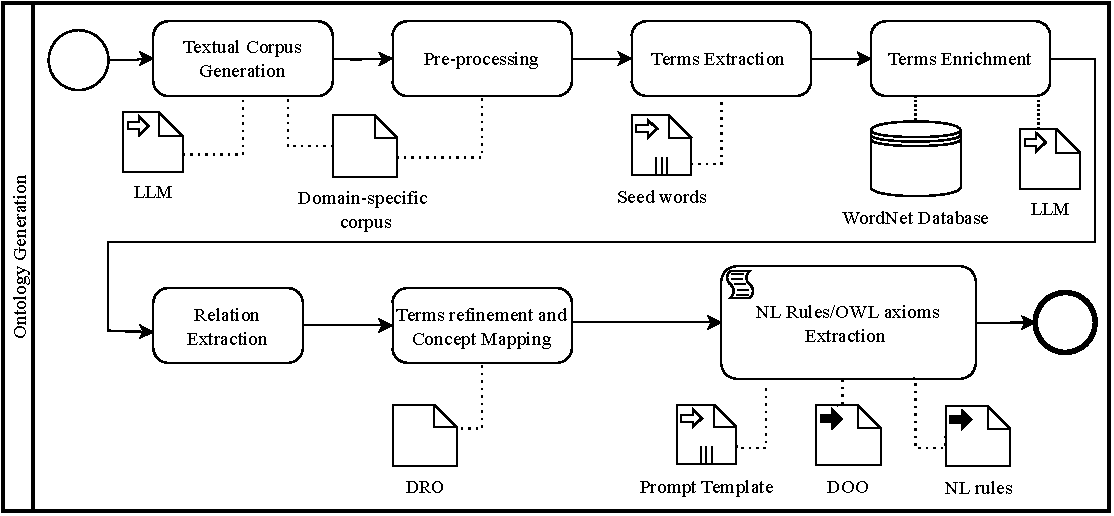
\includegraphics[width=0.85\textwidth]{../figures/MyFigures/OntologyGeneration.drawio.pdf}
\captionsetup{justification=centering}
\caption{Ontology Generation Process}\label{fig:onto-onto-gen}
}
\end{figure}

The input of this process is the domain-related textual corpus. It is essential that the data corpus contains the domain-specific terminological core terms, that completely reflect the domain concepts \autocite{Shams2010}. In a specialized corpus, completeness refers to the extent to which the corpus includes a complete range of domain-specific terms. The domain-specific corpus is generated using \gls{llm} model and input from domain experts, including scenarios and key terms known as seed words. Using seed words guides the concept extraction process later, by helping to identify semantically related concepts. The generated corpus is scenario-driven, allowing for a focused extraction of concepts and relationships relevant to specific situations. 
Pre-processing is an essential step in preparing a corpus for the terms and concepts extraction. This stage involves transforming the unstructured corpus into a structured format to enhance the ontology learning accuracy \autocite{Asim2018}. This process begins by segmentation of the text into sentences and perform the pre-processing steps on each sentence. Key steps involve tokenization, stop word removal, Part of Speech (POS) tagging, parsing, and lemmatization. \cref{fig:onto-Pre-processing}describes the preprocessing steps in detail.  

\begin{figure}[hbt]
\hypertarget{fig:onto-Pre-processing}{%
\centering
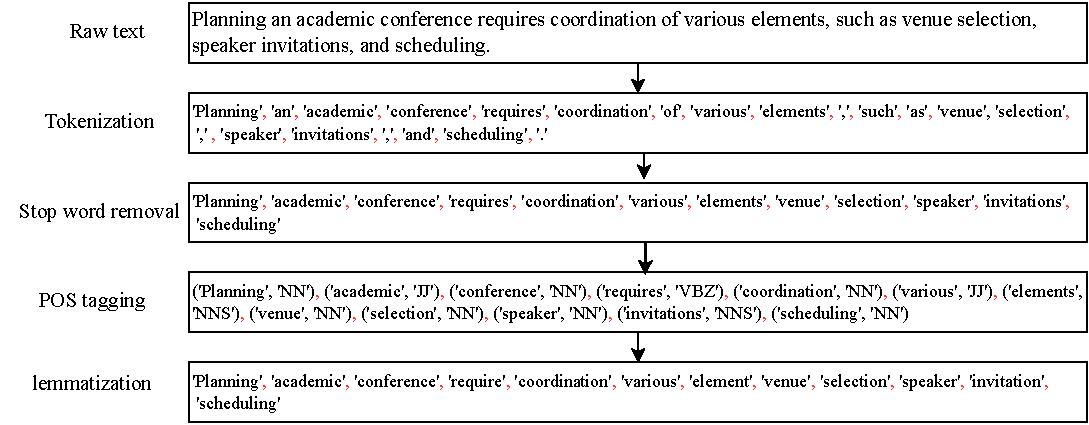
\includegraphics[width=0.85\textwidth]{../figures/MyFigures/Pre-Processing.drawio.pdf}
\captionsetup{justification=centering}
\caption{Pre-processing Steps}\label{fig:onto-Pre-processing}
}
\end{figure}

\emph{Terms Extraction} involves identifying the domain's key terms that
hold significant importance in a specific domain. These terms are then
mapped to corresponding concepts, which are equivalent to the entity
classes within the domain ontology \autocite{Hulth2003}. The method used for
term extraction is a combination of statistical method and linguistic
method. Linguistic-based approaches leverage linguistic information such
as part-of-speech tags and semantic patterns. These techniques are
proved to offer comprehensive and efficient results \autocite{Aman2018}, although they are language-dependent and require domain knowledge
\autocite{Aman2018}, this limitation is mitigated within the
scope of this study, as the domain experts possess the necessary
expertise to address this challenge.

The following algorithm elaborates the term extraction procedure in
detail.

\setlength{\algomargin}{2em} %
\begin{algorithm}
	\DontPrintSemicolon
	\KwIn{Pre-processed corpus}
	\KwOut{\(candicate\_ terms\lbrack\rbrack\) as the list of
	domain's concepts}
	
	\begin{enumerate}
	\item 
	 Run TextRank function with Corpus and
	  \(\mathbf{allowedPOSpatterns\  = \{ NN,\ JJ + \ NN,\ NN + \ NN,\ NN\  + \ IN\  + NN\}}\)
	  as parameters.
	  \item 
	  \ForEach{term extracted by TextRank}
	  			{
	  			\begin{enumerate}
	  				\def\labelenumii{\alph{enumii}.}
	  			\item
	  			  find synonym using WordNet and add to them to
	  			  \(key\_ words\lbrack\rbrack\)
	  			\end{enumerate}
	  			
	  			}\label{endfor}
	  \item 
	  
	   \ForEach{term in \(\mathbf{key\_ words:}\)}
	  	  			{
	  	  		\begin{enumerate}
	  	  			  				\def\labelenumii{\alph{enumii}.}
	  	  			\item
	  	  			 Use HuggingFace hosted LLM to extract semantically related terms and
	  	  			   add them to \(candicate\_ terms\lbrack\rbrack\)
	  	  			\end{enumerate}
	  	  			
	  	  			}\label{endfor}
	  \item
	    Manually validate the \(\mathbf{candicate}\mathbf{\_}\mathbf{terms}\)
	  \item
	    Clustering semantically similar concepts using K-Means algorithm.
	  \item
	    \(\mathbf{Concepts\  = term\_ clusters}\)
	\end{enumerate}
	
\caption{Ontology Concept Extraction}\label{alg:onto-ce}
\end{algorithm}

TextRank is well-suited algorithm for extracting important terms from a
corpus, leveraging co-occurrence patterns and \gls{pos} rules to highlight
relevant noun phrases and compound terms. This algorithm is a
graph-based method inspired by Google\textquotesingle s PageRank, which
ranks web pages in search engines (Hasan and Ng, 2010). This algorithm
models the text as a graph in which every word is correspondence to
vertex \(v_{i}\) and it is connected to vertex \(v_{j}\) with the
weighted edge \(w_{ij}\). The value of \(w_{ij}\) is the number of times
that words \(v_{i}\) and \(v_{j}\ \)are co-occurring within the window
of \(W\) words. The importance of each identified concept in the main
corpus is determined iteratively by the score of each vertex calculated
by the following formula:

\begin{equation}
S(v_{i})\  = \ (\ 1\  - \ d\ )\  + \ d\  \times \ \sum_{v_{j}\  \in \ Adj\ (i)}^{}\frac{w_{ji}}{\sum_{v_{k}\  \in \ Adj\ (v_{j)}}^{}w_{jk}}
\end{equation}

Where \(d\) is the damping factor and the \(Adj\ (v_{i})\) the neighbors
of \(v_{i}\) \autocite{Chuang2012}.

The allowed \gls{pos} patterns for TextRank function is defined as Noun (NN),
Adjective (JJ) + Noun (NN), Noun (NN) + Noun (NN), and Noun (NN) +
Preposition (IN) + Noun (NN). These patterns ensure precision and
performance by limiting the result only to the relevant keywords.

For term enrichment purpose, WordNet\footnote{
  \url{https://wordnet.princeton.edu/}} is used as an external data source to extract associated
terms. WordNet is a large lexical database of synonyms, organized into
groups called synsets, which denote relationships between words. The
enrichment adds extra terms closely related to terms. Further enrichment
is performed by leveraging \gls{llm} model to extract semantically related
terms in the given domain context. \gls{llm}s can provide terms with deeper
semantic similarity and identify concepts that may not be immediately
obvious through TextRank. Therefore, it results in enhanced precision
and enhances the semantic richness.

For the last step, the terms hierarchies are generated by clustering
terms into semantically similar groups. The clustering algorithms are
unsupervised learning approaches which are used to group similar terms
\autocite{Asim2018}. These terms are further refined and expand
during the relation extraction step.

\emph{Relation extraction:} The final step of \gls{dro} generation is
extracting the existing relations among the candidate terms identified
in the previous step. In knowledge engineering, such relations can be
represented as triplet SPO (Subject-Predicate-Object) where the
predicate is a specific relation between two associated entities namely
subject and object \autocite{Li2020}.

To structure the SPO triplets, we use syntactic analysis to extract
subject and object entities related to a predicate (or relation).
Subject and objects can be a simple entity, like "Session" in "Each
session has a keynote speaker." Sentence or a compound entity, such as
"keynote speaker" Compound entities can also consist of more than one
word, such as "Web engineering conference session". To detect compound
entities for a given token\textquotesingle s head, the algorithm
recursively searches for tokens with a "compound" or "amod" dependency
and accumulating all to build a full compound phrase. Algorithm
 describes the process in detail.
 
\setlength{\algomargin}{2em} %
\begin{algorithm}
	\DontPrintSemicolon
	\KwIn{Pre-processed Corpus.txt, \(term\_ candicates\) as a
	list of domain's concepts (\(C_{1}\), \(C_{2}\) \ldots)}
	\KwOut{\(relation\_ list\ \)as List of Tuples (\(C_{m}\),
	relation, \(C_{n}\))}
	
	\begin{enumerate}
	  \item 
	  \ForEach{sentence in Corpus.txt}
	  			{
	  			\begin{enumerate}
	  				\def\labelenumii{\alph{enumii}.}
	  			\item
	  			 Extracts\(\ Subject\) and \(Object\) entities using
	  			   \(getCompoundEntities()\)
	  			\end{enumerate}
	  			
	  			}\label{endfor}
	  \item 
	  If both
	    \({\mathbf{C}_{\mathbf{1}}\mathbf{\ \&\ C}}_{\mathbf{2}}\mathbf{\ }\)
	    are found:
	    \begin{enumerate}
	    \item
	      \(Verb = token.text\ with\ token.dep = = 'ROOT'\)
	    \end{enumerate}
	   
	  \item
	     If \(\mathbf{Subject}\) or \(\mathbf{Object}\) are in the
	      \(\mathbf{term\_ candicates}\) list or similar to the terms in this
	      list:
	      \begin{enumerate}
	      \item
	        \textbf{If} there are any token with \(token.dep\_\  = = \ 'conj'\):
	      
	        \begin{enumerate}
	        \item
	          create a relation for each conjunction. \(Relation\  = \ (subject,\ root\_ verb,\ obj)\)
	        \end{enumerate}
	      \end{enumerate}
	      	    
	 \item
	   \(\mathbf{relation}\mathbf{\_}\mathbf{list}\mathbf{.}\mathbf{append}\mathbf{(}\mathbf{relation}\mathbf{)}\)
	 \item
	   Refine and extend
	   \(\mathbf{relation}\mathbf{\_}\mathbf{list}\mathbf{\ }\)using LLM. \(extract\_ compound\_ entities(sentence)\):
	   
	   \item
	      \ForEach{token in ``sentence'' with token.dep\_== "subj"}{
	     \begin{enumerate}
	     
	     \item
	       Recursively traverse the left children to find compound parts.
	     \item
	       Append each compound part and return the full compound phrase as
	       \(Subject\) entity.
	     \end{enumerate}
	     }\label{endfor}
	     
	     
	     \item
	     	      \ForEach{token in ``sentence'' with token.dep\_== "obj" or ``attr''}{
	     	     \begin{enumerate}
	     	     
	     	     \item
	     	       Recursively traverse the left children to find compound parts.
	     	     \item
	     	       append each compound part and return the full compound phrase as
	     	       \(Object\) entity.
	     	     \end{enumerate}
	     	     }\label{endfor}
	     
	\end{enumerate}
	
\caption{Ontology Generation- Relation Extraction}\label{alg:onto-re}
\end{algorithm}

\emph{Terms refinement and concept mapping:} once the \(RelationList\)
is generated, it\textquotesingle s crucial to thoroughly refine the list
of candidate terms. According to Algorithm 7.2,
the subjects and objects of the generated triplets are included in the
\(TermCandidates\) list. Any terms that are not associated with a
relation, should be removed from the \(TermCandidates\). For each
remaining term, a corresponding class will be created to represent a
domain concept. The identified relations will be represented as object
properties connecting two concepts.

\emph{Rules extraction and axiom mapping:} during this step, the domain
business logic, also known as domain business rules, is extracted.
Domain rules are set of constraints controlling the domain in a
declarative manner \autocite{Kalibatiene2010}. These rules are
essential for defining the necessary domain customizations required by
domain experts. In ontology-driven development, domain business rules
are expressed as ontology axioms, which define the relationship
constraints and interpret the domain concepts \autocite{DeFreitas2022}). In the software ecosystem, rules are defined in one of the
following forms:

\textbf{Formal rules} are defined using an executable formal language
such as \gls{sql} or declarative rule languages such as \gls{swrl} or \gls{ocl}.

\textbf{Template-based rules} are predefined rules that use decision
tables or decision trees to express informal rules. The executable rules
are generated based on these template-based rules.

\textbf{NL rules} are defined in natural language as guidance for users
\autocite{Kalibatiene2010}.

To efficiently generate domain business rules, we leveraged \gls{llm}s. The
initial step in employing \gls{llm}s involves \textbf{prompt engineering},
which refers to generating structured prompt templates to guide \gls{llm}s
toward more accurate answers. A method in prompt engineering is the
\textbf{\gls{cot}}, which breaks down complex problems into
smaller, more manageable questions, encouraging the model to follow a
step-by-step reasoning. Another technique is \emph{few-shot} method
which involves providing input-output examples allowing the \gls{llm} to learn
the desired structure and produce a consistent response. On the other
hand, the zero-shot method just provides the task description without
any example of input or output data \autocite{Crum2024}.

An example of prompt template is presented in Appendix . This template
structured to extract business rules in the ``Academic planning''
scenario (c.f. \cref{sec:scenario}) using Hugging Face API\footnote{\url{https://huggingface.co/}}.
Although this prompt does not provide explicit examples, it does outline
a structured process that resembles few-shot prompting in its
instructional nature.

The prompt instructs the \gls{llm} to extract business rules in in two
formats: natural language for integration with the UI, and RDF/XML for
incorporation into the OWL ontology. The category determines whether the
rule should be enforced in the backend or the UI. Two categories are
defined accordingly:

\begin{itemize}
\item
  \({RL}_{C}\  = \ \{{rl}_{ci}\}\) being set of rules as Composition
  Model restrictions for allowing or denying component coupling.
\item
  \({RL}_{G} = \ \{{rl}_{gi}\}\) being set of NL-based rules as
  assistance during the runtime.
\end{itemize}

Restriction rules define the cardinality and structure of the
relationships among the concepts. Restrictions such as
\(owl:minCardinality\),\(\ owl:maxCardinality\), and \(owl:cardinality\)
fit in the backend to enforce the structural constraint to ensure data
integrity.

Assistance rules are best suited for the UI, where they can be displayed
as recommendations without being strictly enforced in the ontology.

The extraction process relies on the concepts and relationships
identified during the term and relation extraction phases. The language
model used for this purpose is the pre-trained and fined-tuned
Zephyr-7B-$\beta$\footnote{https://huggingface.co/HuggingFaceH4/zephyr-7b-beta}.
This model demonstrated strong performance on several categories such as
text generation, extraction, and STEM. The model performance in these
categories is the same as GPT-4 or GPT-3.5-turbo. Following some
examples of extracted business rules and their corresponding RDF is
given.

\textbf{Business Rule 1}: \emph{"A Keynote Speaker can only speak at one
Session at a time"}.

\textbf{RDF/XML:}
\begin{lstlisting}[language=JavaScript, captionpos=t, caption=Example of a bussiness rule XML/Rdf]
<owl:Class rdf:about="#KeynoteSpeaker">
    <rdfs:subClassOf>
        <owl:Restriction>
            <owl:onProperty rdf:resource="#holds"/>
            <owl:maxCardinality rdf:datatype="#nonNegativeInteger">1 
   </owl:maxCardinality>
        </owl:Restriction>
    </rdfs:subClassOf>
</owl:Class>
\end{lstlisting}

\textbf{Business Rule 2}: \emph{"Research related to a research interest must
be presented at a conference with a focus on Web Engineering."}

\textbf{RDF/XML:}

\begin{lstlisting}[language=JavaScript, captionpos=t, caption=Example of a bussiness rule XML/Rdf]
<owl:Class rdf:about="#Research">
      <rdfs:subClassOf>
        <owl:Restriction>
          <owl:onProperty rdf:resource="#isRelatedTo"/>
          <owl:someValuesFrom rdf:resource="#ResearchInterest"/>
          <owl:onProperty rdf:resource="#isPresentedAt"/>
          <owl:someValuesFrom>
            <owl:Class rdf:about="#Conference">
              <owl:Restriction>
                <owl:onProperty rdf:resource="#isFocusOf"/>
                <owl:someValuesFrom rdf:resource="#WebEngineering"/>
              </owl:Restriction>
            </owl:Class>
          </owl:someValuesFrom>
        </owl:Restriction>
      </rdfs:subClassOf>
    </owl:Class>

\end{lstlisting}

\textbf{Business Rule 3}: \emph{"For better networking opportunities, schedule
social events during lunch breaks or at the end of the conference day."}

\textbf{RDF/XML:} This is assistance rule. No Owl available.

\textbf{Business Rule 4}: \emph{"Generate an agenda for each session based on
the duration and number of speakers."}

\textbf{RDF/XML:} This is assistance rule. No Owl available.

\vspace{-15pt}
\hypertarget{sec:onto.dc}{%
\subsection{Domain Configuration}\label{sec:onto.dc}}
\vspace{10pt}

According to BPMN presented in \cref{fig:onto-da}, the subsequent step involves
implementing domain-specific customizations within the DSAC tool. This
configuration process occurs at three distinct levels: the component
level, the composition level, and the UI level.

To apply the component and composition level customization, the first
step is to semantically annotate the components using \gls{dro}. The method
used for this purpose is inspired by the Semantic Table Interpretation
(STI) algorithm \autocite{Huynh2023}. Each component in the
component repository is represented as a row, accompanied by metadata
such as a unique identifier, name, and description. Additionally, a
field for semantic annotation is included to store the component's
semantic data (refer to component model in \cref{fig:component-model}). The annotation
provides a reference to the domain ontology identified as the component
target domain, as well as the specific concept to which the component is
linked. The mapping process relies on assessing semantic similarity
between the component's name and description and concepts in the domain
ontology. The resulting annotations are further enriched and refined
using large language models (\gls{llm}s). At the component level, the
annotations are used for component discovery to retrieve domain-specific
components. At the composition level, the restriction rules extracted
during the ``Rules extraction and axiom mapping'' step are integrated
into the composition model as communication restrictions which is
applied to the components involving in the composition.

Since components can belong to multiple domains, each can refer to more
than one domain and may include several semantic annotations. Following
algorithm describe the mapping process:

% % Algo
At the UI level, the assistance business rules are integrated into the UI to assist and guide domain experts during the composition process.


\vspace{-15pt}
\hypertarget{sec:onto.evaluation}{%
\section{Evaluation}\label{sec:onto.evaluation}}
\vspace{10pt}
The evaluation process presented in this section assesses the domain Analyzer’s performance in addressing the “Limited domain specificity” sub-problem to achieve \cref{ro:3}. The quality of the domain customizations can be evaluated at different levels, with the quality of the generated ontologies playing a central role. The ontologies are evaluated for coverage at the concept level, the correctness of extracted relations, and accuracy of business rules. 
The ontology evaluation is a complex task and an ongoing field of research. Numerous techniques have been proposed to assess ontologies based on specific criteria. These methods are mainly categorized into four groups: golden standard-based, Corpus-based, application-based, and human evaluation. Selecting an appropriate method is subjective and depends on the evaluation criteria relevant to the intended application of the ontology. In line with the overall objective and particularly \cref{ro:3} concerning ontology-based configuration mechanism, we employed data-driven and human evaluation approaches to assess the two \gls{dro} and \gls{doo} ontologies.

\vspace{-15pt}
\hypertarget{sec:onto.evaluation-data}{%
\subsection{Data-driven Evaluation}\label{sec:onto.evaluation-data}}
\vspace{10pt}

The quality of generated ontologies was evaluated across three distinct domains. For each domain, we generated a sample textual corpus using a \gls{llm} trained on publicly available datasets, such as Wikipedia and online articles. After preprocessing the text with Python libraries such as Spacy and NLTK, the corpus is ready for terms/concepts extraction. These steps were guided by seed words provided by participants recruited specifically for evaluation tasks (c.f. \cref{sec:disco-evaluation}). 

\textbf{Result}

\cref{tbl:eval.generated-ontologies} presents the results of ontology generation, detailing the
number of terms, relations, and business rules generated across three
distinct domains: academia, travel, and online shopping. The number of
extracted relations and rules were calculated following a manual
refinement process the concepts and removing the unrelated ones.

\hypertarget{tbl:eval.generated-ontologies}{}
\begin{longtable}{@{}lccc@{}}
\caption{\label{tbl:eval.generated-ontologies}Generated Ontologies Statistics}\tabularnewline
\toprule
\begin{minipage}[b]{0.32\columnwidth}\raggedright
\end{minipage} & 
\begin{minipage}[b]{0.22\columnwidth}\centering
\textbf{Academic}\strut
\end{minipage} & 
\begin{minipage}[b]{0.22\columnwidth}\centering
\textbf{Travel}\strut
\end{minipage} & 
\begin{minipage}[b]{0.24\columnwidth}\centering
\textbf{Online Shop}\strut
\end{minipage} \tabularnewline
\midrule
\endfirsthead

\toprule
\begin{minipage}[b]{0.32\columnwidth}\raggedright
\end{minipage} & 
\begin{minipage}[b]{0.22\columnwidth}\centering
\textbf{Academic}\strut
\end{minipage} & 
\begin{minipage}[b]{0.22\columnwidth}\centering
\textbf{Travel}\strut
\end{minipage} & 
\begin{minipage}[b]{0.24\columnwidth}\centering
\textbf{Online Shop}\strut
\end{minipage} \tabularnewline
\midrule
\endhead

Extracted Terms & 33 & 20 & 24 \tabularnewline
Extracted Relations & 22 & 11 & 14 \tabularnewline
Rules & 8 & 5 & 4 \tabularnewline

\bottomrule
\end{longtable}

Based on the above data, the  precision and recall are presented in the table below. For each domain two metrics were calculated for terms and relations extraction. 

\hypertarget{tbl:eval.term-extraction}{}
\begin{longtable}{@{}lccc@{}}
\caption{\label{tbl:eval.term-extraction}Evaluation Result for Term Extraction}\tabularnewline
\toprule
\begin{minipage}[b]{0.30\columnwidth}\raggedright
\textbf{Metric}\strut
\end{minipage} & 
\begin{minipage}[b]{0.23\columnwidth}\centering
\textbf{Academic}\strut
\end{minipage} & 
\begin{minipage}[b]{0.23\columnwidth}\centering
\textbf{Travel}\strut
\end{minipage} & 
\begin{minipage}[b]{0.24\columnwidth}\centering
\textbf{Online Shop}\strut
\end{minipage} \tabularnewline
\midrule
\endfirsthead

\toprule
\textbf{Metric} & \textbf{Academic} & \textbf{Travel} & \textbf{Online Shop} \tabularnewline
\midrule
\endhead

Precision & 72.7\% & 80\% & 87.5\% \tabularnewline
Recall & 88\% & 100\% & 100\% \tabularnewline

\bottomrule
\end{longtable}

\hypertarget{tbl:eval.relation-extraction}{}
\begin{longtable}{@{}lccc@{}}
\caption{\label{tbl:eval.relation-extraction}Evaluation Results for Relation Extraction}\tabularnewline
\toprule
\begin{minipage}[b]{0.30\columnwidth}\raggedright
\textbf{Metric}\strut
\end{minipage} & 
\begin{minipage}[b]{0.20\columnwidth}\centering
\textbf{Academic}\strut
\end{minipage} & 
\begin{minipage}[b]{0.20\columnwidth}\centering
\textbf{Travel}\strut
\end{minipage} & 
\begin{minipage}[b]{0.20\columnwidth}\centering
\textbf{Online Shop}\strut
\end{minipage} \tabularnewline
\midrule
\endfirsthead

\toprule
\begin{minipage}[b]{0.30\columnwidth}\raggedright
\textbf{Metric}\strut
\end{minipage} & 
\begin{minipage}[b]{0.20\columnwidth}\centering
\textbf{Academic}\strut
\end{minipage} & 
\begin{minipage}[b]{0.20\columnwidth}\centering
\textbf{Travel}\strut
\end{minipage} & 
\begin{minipage}[b]{0.20\columnwidth}\centering
\textbf{Online Shop}\strut
\end{minipage} \tabularnewline
\midrule
\endhead

Precision & 91\% & 90\% & 87\% \tabularnewline
Recall & 90\% & 90\% & 100\% \tabularnewline

\bottomrule
\end{longtable}

According to the result presented here, a resalable precision and recall scores were obtained during the Domain Analyzer evaluation. These results demonstrated improved precision for relation extraction following a manual terms refinement process. To justify the false positives rate (incorrectly extracted relations), some examples such as (Accommodation, enhance, Experience), are semantically valid but they removed because they do not provide precise meaning when mapped into components. 
Moreover, it is important to highlight that integrating \gls{llm}s in ontology learning process, significantly enhances the result of terms and relation extraction compared to relying solely on the conventional NLP-based methods. Although \gls{llm}s are proved to be efficient, they are particularly effective when using as for refinement and extension purposes  following the application of NLP methods.



\vspace{-15pt}
\hypertarget{sec:onto.evaluation-user}{%
\subsection{User Study Evaluation}\label{sec:onto.evaluation-user}}
\vspace{10pt}

A dedicated user study assesses the extent to which the Domain Analyzer fulfils the "Usability" requirement \cref{tr:1} and the "Interactive User Interface" requirement (TR1) outlined in \cref{sec:requirements}. For this purpose, we assigned specific tasks to five participants. Each task was designed to reflect a distinct aspect of the mentioned requirements. Participants were selected randomly from the 15 test subjects that were already discussed in \cref{sec:disco-evaluation-disco}. The average of user’s rating  on a 5-point Likert scale, determines the usability properties.
The evaluation process begins by a short tutorial to familiarize participants with the platform general concepts and objectives. Then each participant was assigned a specific domain, accompanied by a brief description of the domain and the relevant problem context. As the final step, participants filled out a questionnaire to assess the platform's usability properties.

\textbf{Task 1: Initial navigation and Basic Ontology Creation}

In this task, participants were instructed to navigate the platform
independently, using only the assistance features provided by the
platform. The objective was to generate an ontology of the specific
domain.

\textbf{Motivation:} This task aims at assessing the \emph{learning
curve} and readability within the platform, reflecting the platform's
usability. Time and effort spent by participants to understand the
layout and interaction patterns provides useful insight into how
intuitive and user-friendly the platform is.

\textbf{Task 2: UI Interaction and Interface Features}

In this task, participants were instructed to interact with the platform
using natural language and UI elements. The objective was prompting
participants to try different ways of generating ontology either by
describing the problem scenario or specifying the ontology elements.

\textbf{Motivation}

This task evaluates the "Interactive User Interface" requirement (TR1),
focusing on natural language support and overall interactivity. The
evaluation offers insights into the platform's responsiveness and
interactive functionalities.


\cref{fig:onto.eval.ss1} and \cref{fig:onto.eval.ss2} present screenshots of the platform during the
ontology generation process, highlighting key features in real-time
usage. The platform provides step-by-step instructions to guide
participants through the process. Additionally, the built-in assistance
features, such as tooltips, enhance user support and clarity.

\begin{figure}[hbt]
\hypertarget{fig:onto.eval.ss1}{%
\centering
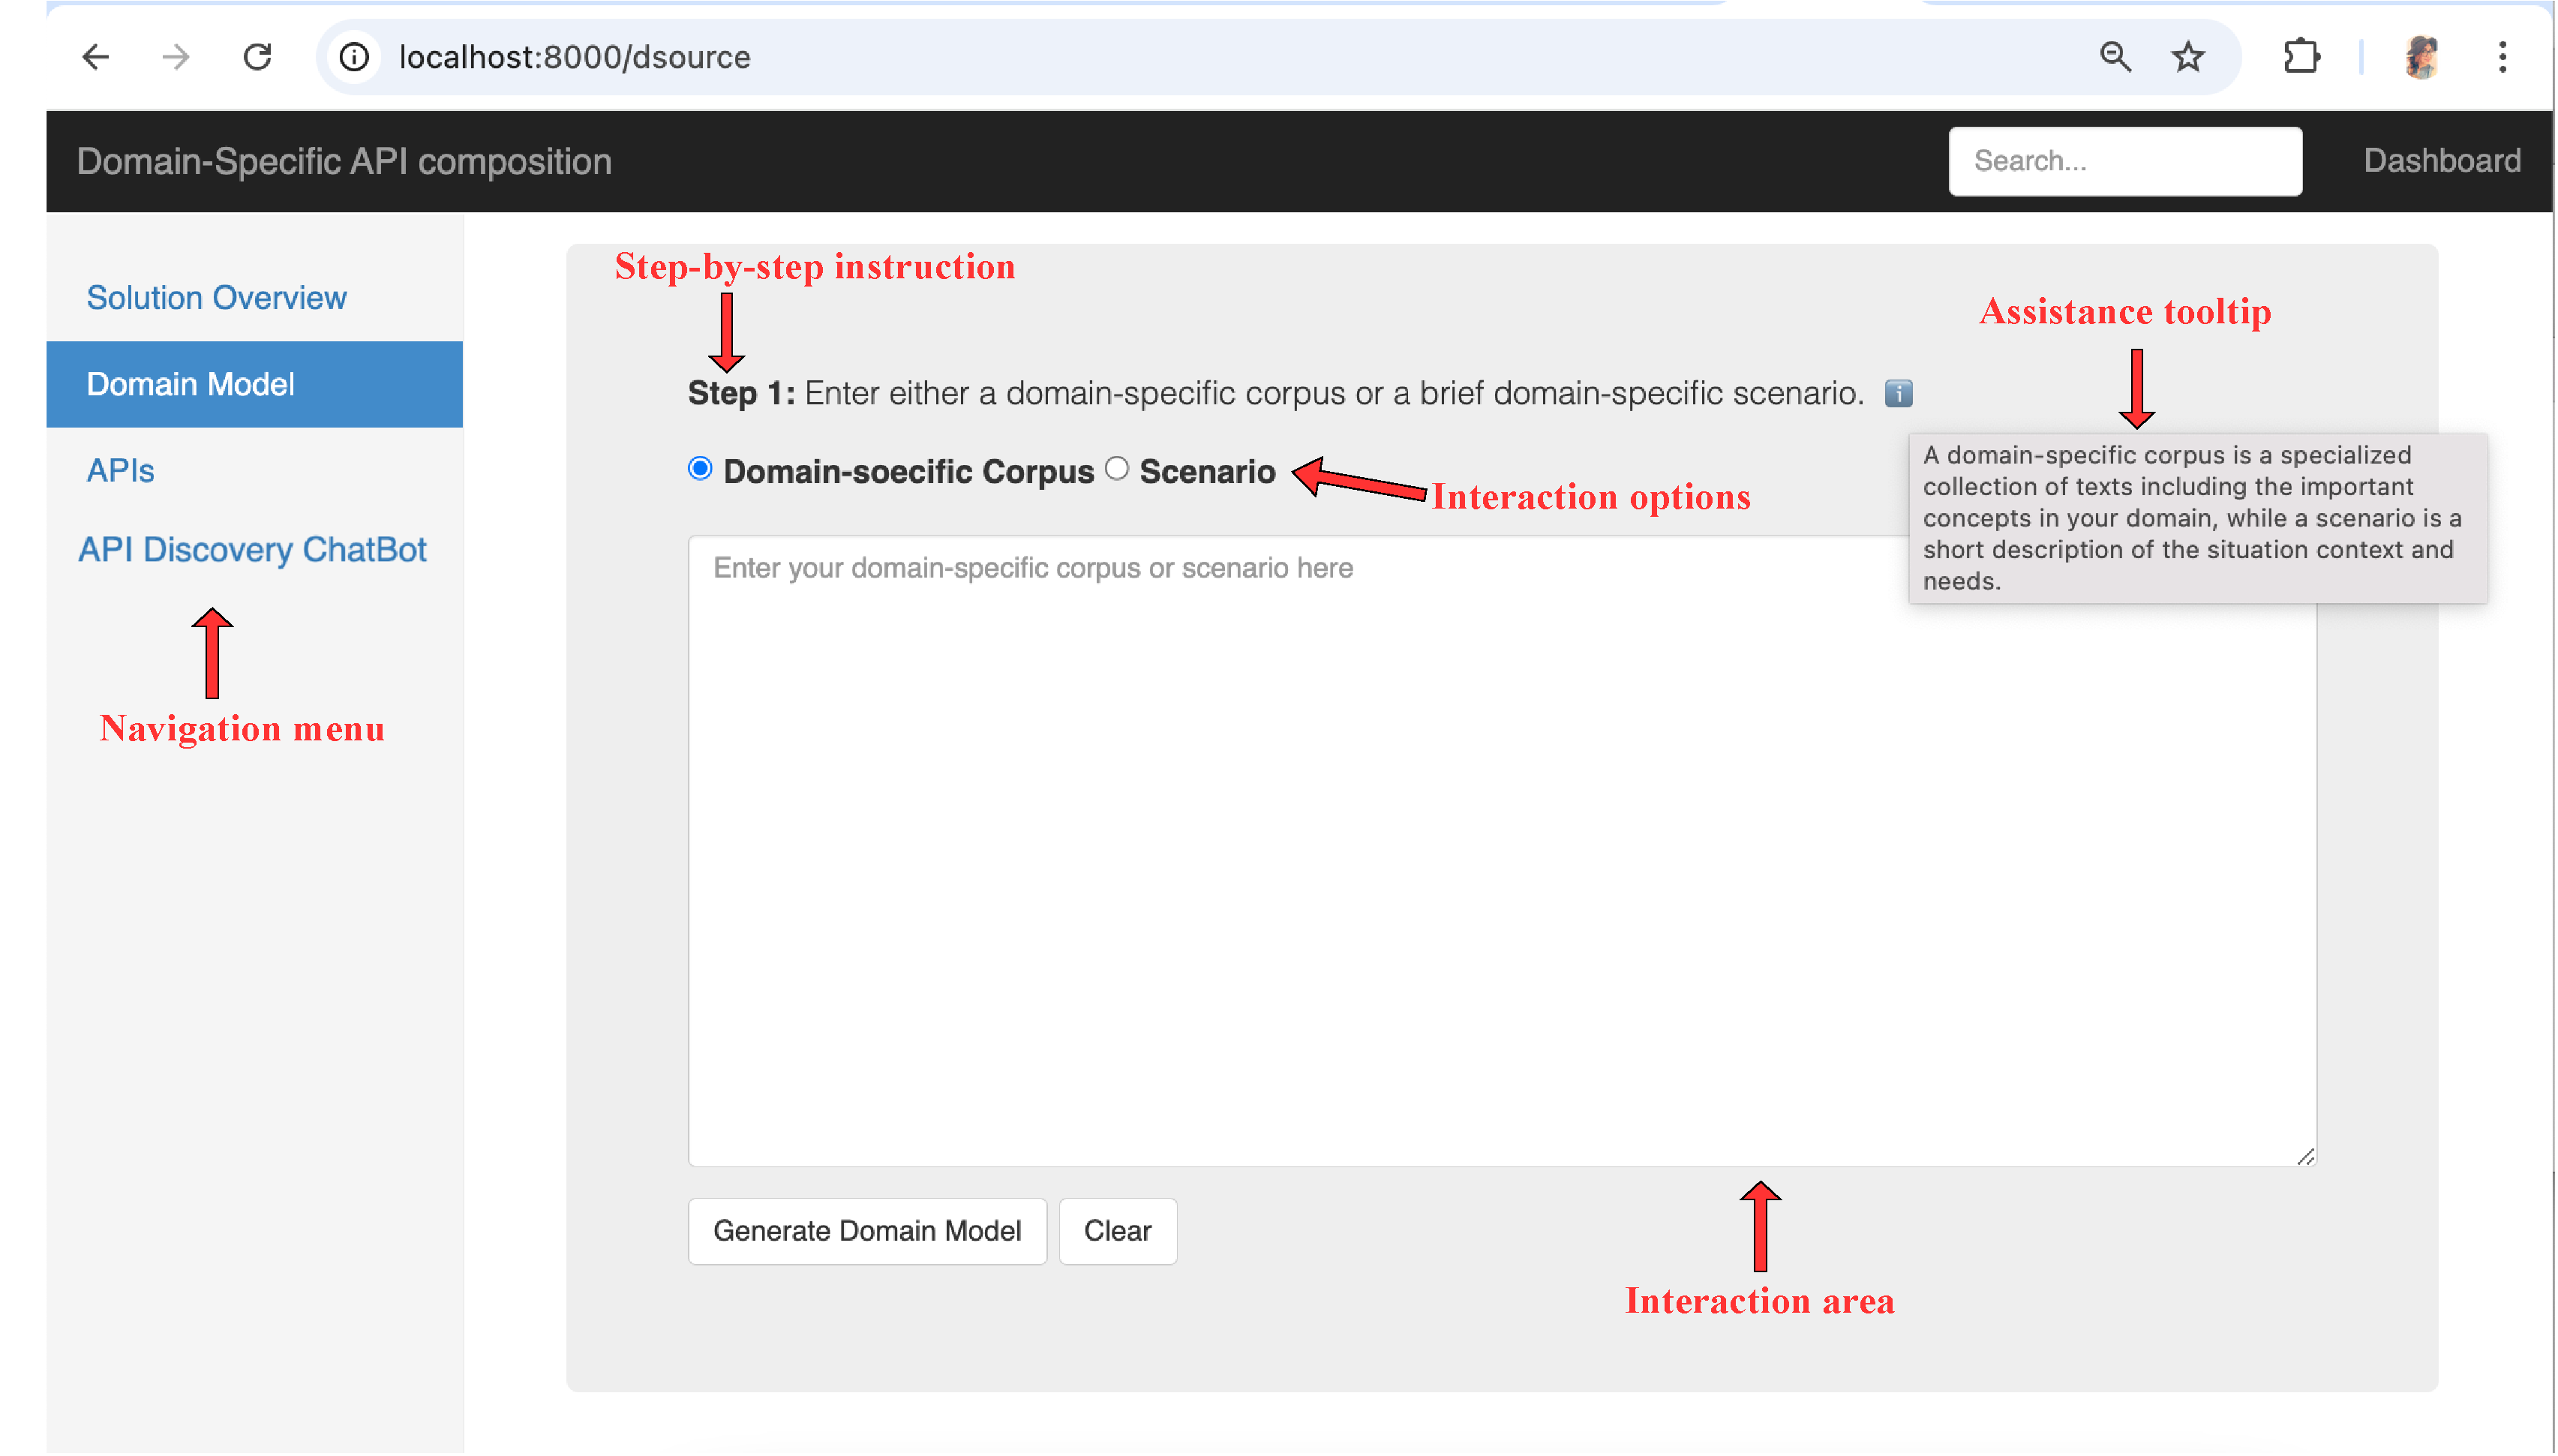
\includegraphics[width=0.85\textwidth]{../figures/MyFigures/ScreenshootNew.drawio.pdf}
\captionsetup{justification=centering}
\caption{Screenshot of Ontology Generation Process}\label{fig:onto.eval.ss1}
}
\end{figure}

\begin{figure}[hbt]
\hypertarget{fig:onto.eval.ss2}{%
\centering
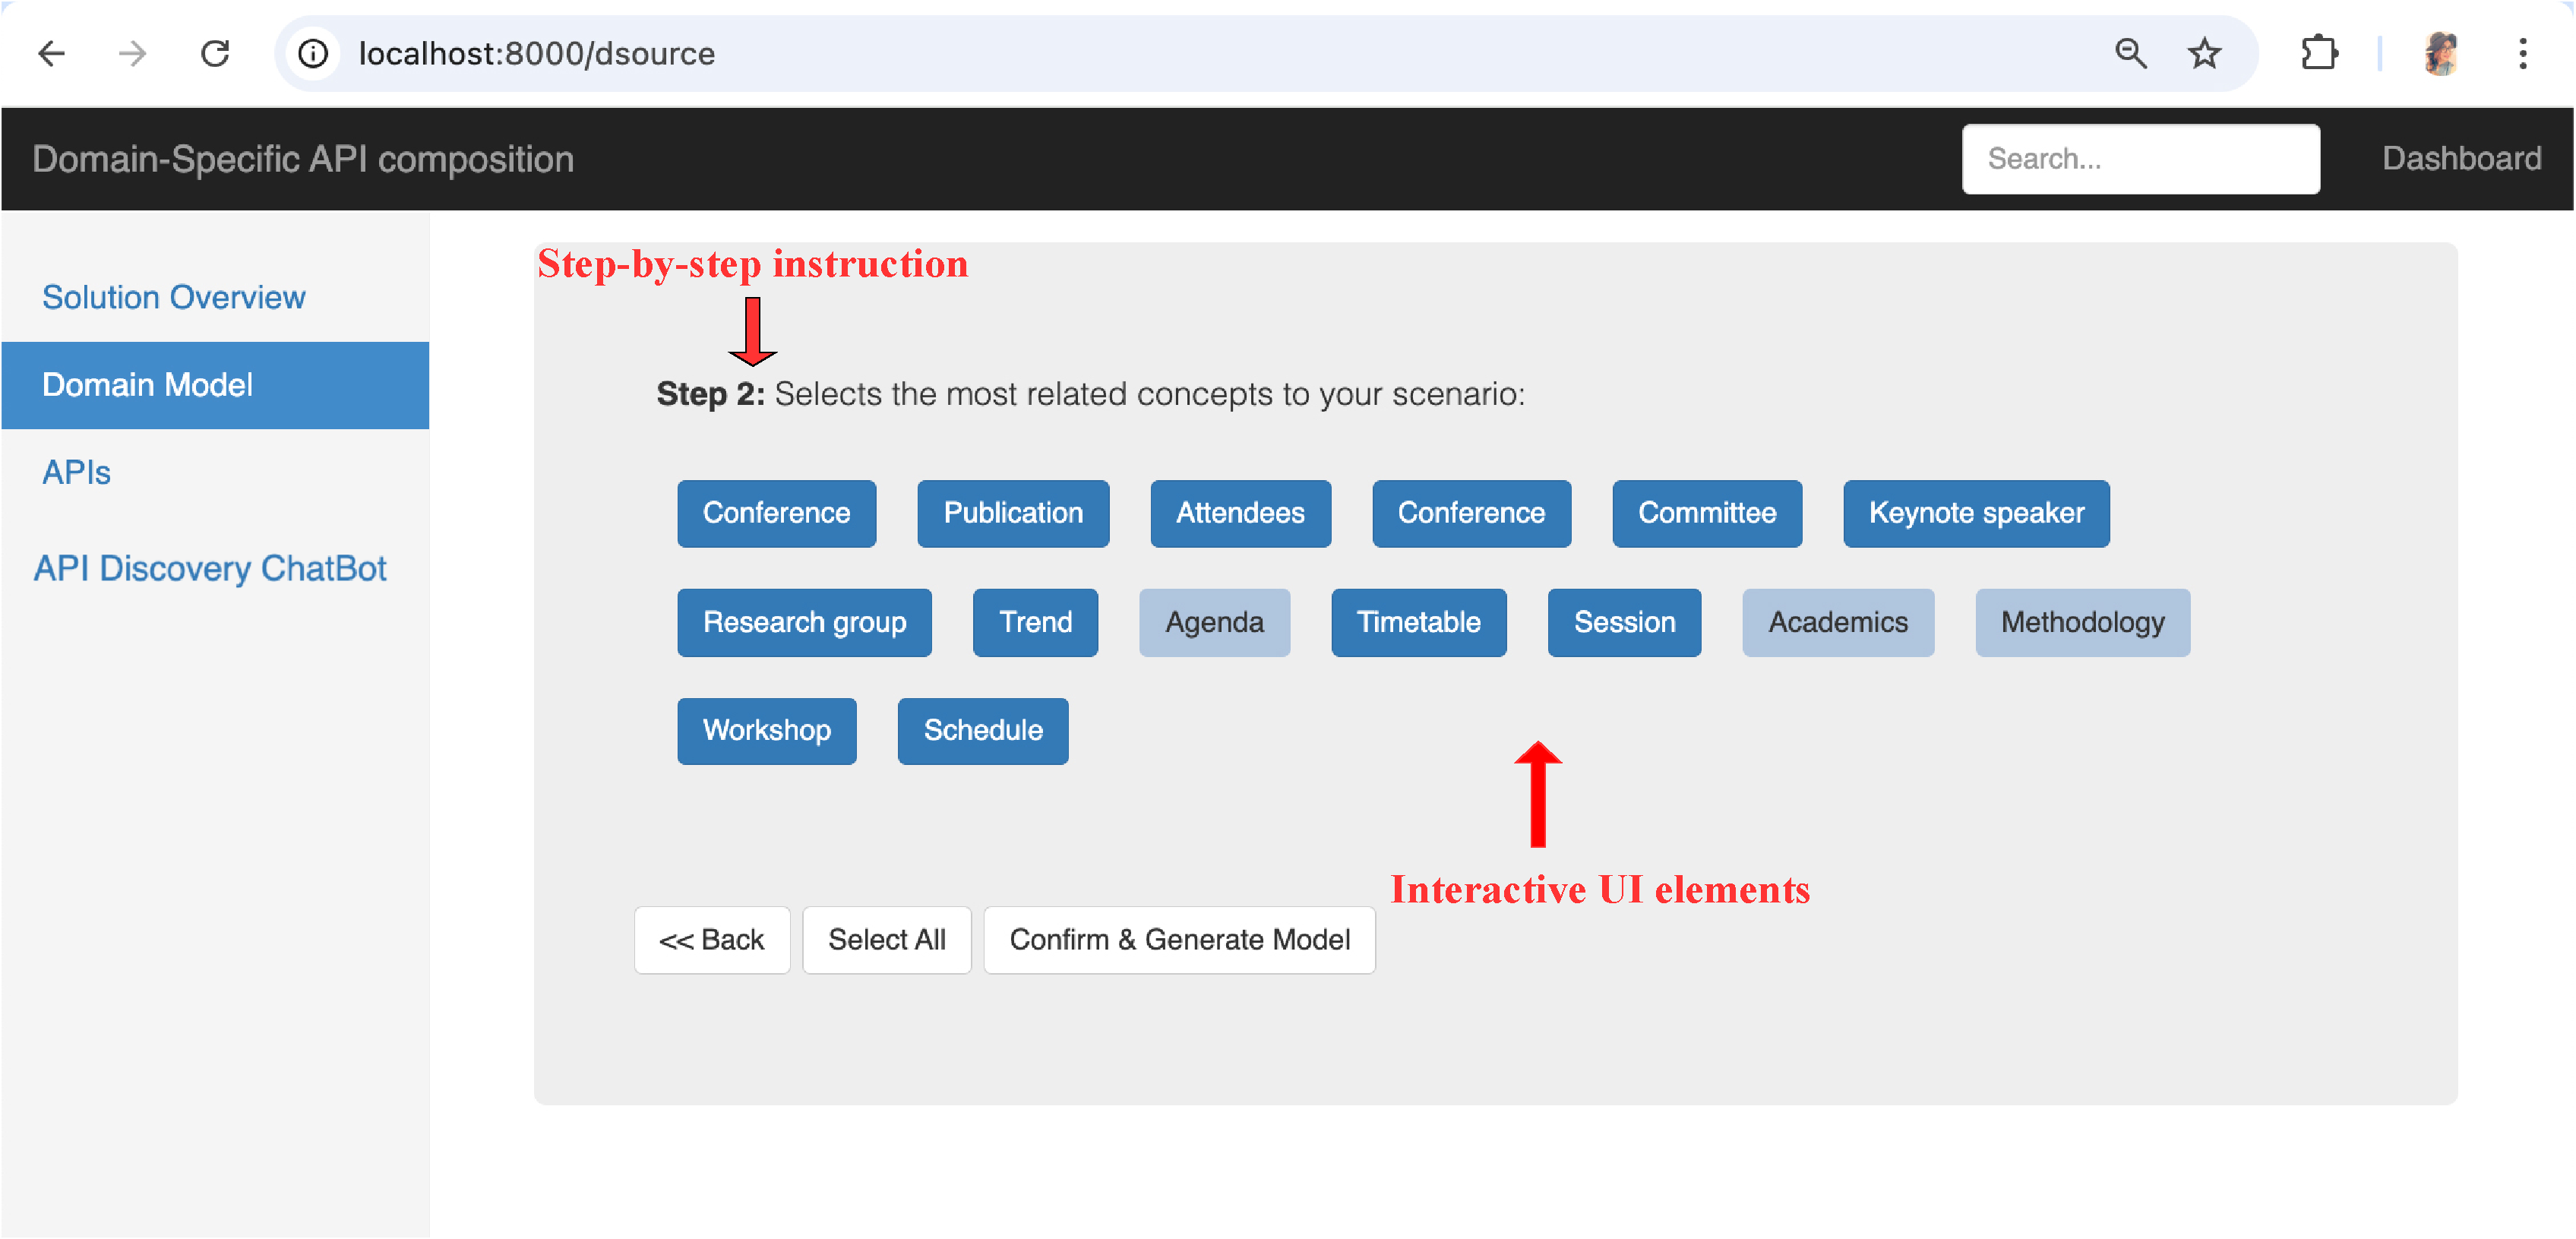
\includegraphics[width=0.85\textwidth]{../figures/MyFigures/Ontologygenerationsceenshot.drawio.pdf}
\captionsetup{justification=centering}
\caption{Screenshot of Ontology Generation Process Step 2}\label{fig:onto.eval.ss2}
}
\end{figure}

The post-task questionnaires (refer to Appendix) were filled by the participants immediately after the task completion. These questionnaires included questions to evaluate different aspects of usability, depending on the assessment criteria. For each task participants were asked different questions reflecting their experience. 


\subsubsection*{Result}
All participants successfully managed to generate the ontology without
the need for further assistance. Analysis of the questionnaire shows
that 80\% of participants rated the platform\textquotesingle s usability
as "Good" while 20\% rated it as "Excellent". This distribution of
responses suggests a strong overall usability performance. Other ratings
indicate that the platform\textquotesingle s readability and ease of
learning were favorable, with 40\% of participants rating it as "Easy"
and another 40\% as "Extremely Easy." Additionally, the UI elements
designed to assist users performed well, as 60\% of participants found
the platform "Extremely Easy" to navigate and use.

The second questionnaire evaluated the effectiveness of the platform's
interactive UI in meeting the "Interactive User Interface" requirement.
In this assessment, 60\% of participants rated the
platform\textquotesingle s user interface as excellent and 40\% as good
in supporting natural language-based interactions.

Based on the findings of the evaluation process, the Usability
requirement is fully satisfied.


\vspace{-15pt}
\hypertarget{sec:onto.summary}{%
\section{Summary}\label{sec:onto.summary}}
\vspace{10pt}

This chapter presented the final piece of DSAC toolkit, designed to achieve \cref{ro:3} by addressing the “Limited domain specificity” problem. The Domain Analyzer, introduced in this chapter, is responsible for integrating a semantic layer within the platform to embeds domain-specific concepts and rules across the component, composition, and UI levels through an ontology-based approach. The proposed approach consists of two key phases: Ontology Generation and Domain Configuration. For Ontology Generation, a hybrid approach is employed, combining lexical-syntactic patterns and statistical techniques. To further improve outcomes, this approach integrates LLMs to enhance the relation and rules extraction. Evaluation of this approach, detailed in \cref{sec:onto.evaluation}, includes data-driven analysis and user studies, both of which demonstrate promising results. 